\documentclass{beamer}
\usetheme{metropolis} 
\usecolortheme{rose}

\usepackage{tikz}
\usepackage{multicol}

\hypersetup{unicode=true}
\usepackage[normalem]{ulem}  % для зачекивания текста

\usepackage{xcolor}
\usepackage[utf8]{inputenc}
\usepackage{hyphenat}
\usepackage[russian,english]{babel}          % Use metropolis theme
\usepackage{wrapfig}

\setbeamertemplate{footline}[frame number] % указывает на каждой странице общее количество страниц

% Указывайте все новые термины в \termdef команде. А уже известные ранее или из других курсов в \term
\newcommand{\termdef}[1]{\textbf{\textit{#1}}}
\newcommand{\term}{\textit}
% Диалог с аудиторией.
\newcommand{\auditorium}[1]{\color{red}{\textbf{#1}}}
% \setbeamercolor{auditorium}{fg=red}

\title{Лекция 3. Дерево решений. Лес. Случайный лес}
% \date{\today}
\date{1 октября 2019}
\author{Павел Владимирович Слипенчук}
\institute{Москва, МГТУ им.Бауманка,\\ каф.ИУ-8, КИБ}
% \titlegraphic{\includegraphics[width=2cm]{logo_ur.jpg}}
\titlegraphic{\small \href{https://github.com/kib-courses/dsis}{Data Science для решения задач информационной безопасности}}

\begin{document}
  \maketitle
    
  \begin{frame}{План лекции}
    \begin{enumerate}
	 \item \nameref{section:tree_forest}
	 \item \nameref{section:random_tree_building}
	% \item \nameref{section:precision_recall_defs}
	% \item \nameref{section:all_of_them}
	\end{enumerate}
 \end{frame}
    
  \begin{frame}
  \begin{block}{Замечание}
  	Алгоритмов машинного обучения очень много. 
  	Хороший Data Scientist должен взять себе в привычку
  	время от времени изучать те или иные алгоритмы.
  	
  	Цель курса -- прикладная. Научить решать ИБ задачи с помощью
  	Data Science методов.
  	
  	Тем не менее хотя бы один алгоритм должен быть изучен.
  \end{block}
 \end{frame}
  \begin{frame}
  \termdef{Случайный лес}(Random Forest, RF) -- это легко объясняемый, 
  понятный, 
  устойчивый к переобучению (overfitting)
  алгоритм ML.
  
  RF является мощным средством против <<активного противника>>\footnote{
  в задачах с обратной связью изучаемого субъекта (хакера, мошенника)
  }. 

  Вопреки высасаным из пальца примерам, на реальныхъ данных
  RF всегда работает, если признаки информативны и "неразряжены".
  \end{frame}

   \section{Дерево решений. Лес решений}\label{section:tree_forest}
	

  \begin{frame}{Дерево решений}
  
  Отрывок из <<Choosing the right estimator>>:\footnote{\tiny \url{https://scikit-learn.org/stable/tutorial/machine_learning_map/index.html}}
  \begin{center}
  	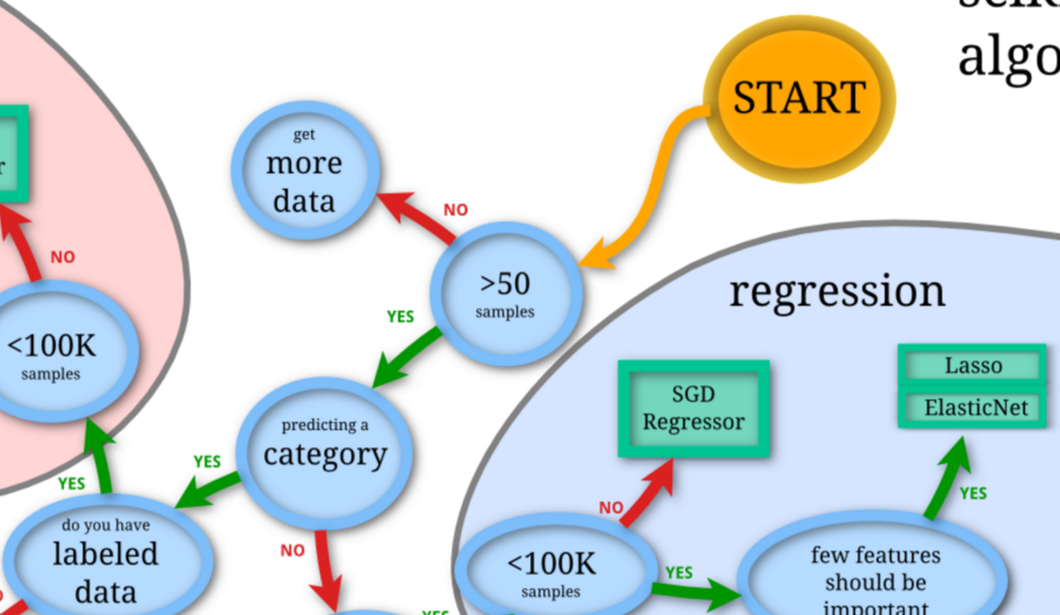
\includegraphics[width=6.5cm]{../pic/scikit_desicion_tree.png}\centering
  \end{center}
  На каждом шаге мы отвечаем на вопрос и "идем по дереву дальше".
  \end{frame}

  \begin{frame}{Пример дерева решений: <<Ирисы Фишера>>}
  \begin{center}
  	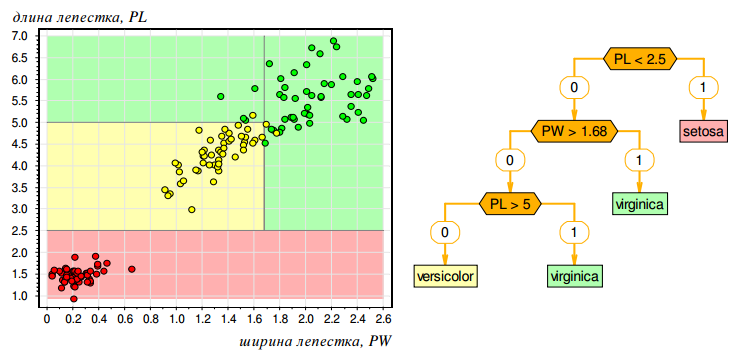
\includegraphics[width=11cm]{../pic/fisher_iris_tree.png}
  \end{center}
  Пример \term{экспертной системы}, являющийся решающим деревом.
  \end{frame}

  \begin{frame}{Пример дерева решений: <<Ирисы Фишера>>}
  
   \begin{center}
  	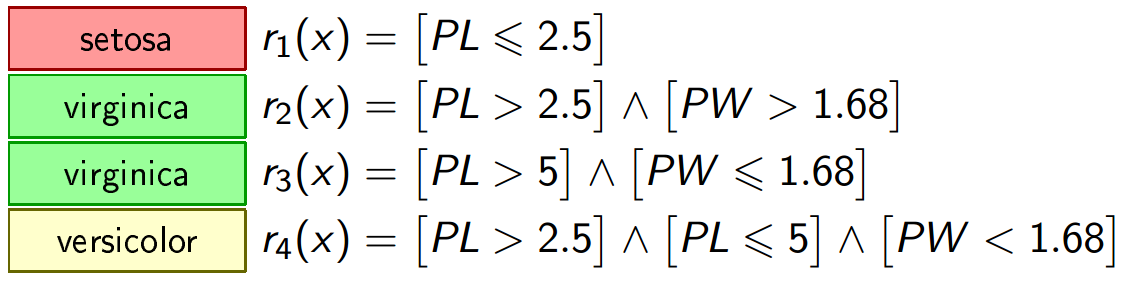
\includegraphics[width=11cm]{../pic/fisher_iris_boolean.png}
  \end{center}
  
  Любое \term{дерево решений} можно представить в виде совокупности
  булевых выражений.
  \end{frame}

  \begin{frame}{Формальное определение}
  
  \termdef{Дерево} -- это \fbox{связанный} \fbox{ациклический} \fbox{граф}.
  
  \termdef{Дерево решений} -- это \fbox{дерево}, в терминальных вершинах которых 
  определён \term{отклик}, в остальных \fbox{листьях} -- функции\footnote{
  	на практике -- \term{булевые} функции, но в общем определении -- не обязательно.}
  каждый выход из которых определяет метку какого-либо выходящего \fbox{ребра}.
  \end{frame}

  \begin{frame}{Лес решений.}
  \termdef{Лес решений} -- это \term{ансамбль}, каждый классификатор которого 
  является \term{деревом решений}.
  
  Обычно лес решений -- это среднее арифметическое всех его деревьев. 
  
  Например решаем задачу обнаружения мошенничества. Всего обучено 500 деревьев решений.
  На какой-либо транзакции 423 дерева определили что эта транзакция мошенническая,
  42 -- легитимная, остальные 35 деревьев -- отказ от классификации.
  
  \auditorium{Каков отклик данного леса?}
  \end{frame}

    \begin{frame}{Лес решений.}
  \termdef{Лес решений} -- это \term{ансамбль}, каждый классификатор которого 
  является \term{деревом решений}.
  
  Обычно лес решений -- это среднее арифметическое всех его деревьев. 
  
  Например решаем задачу обнаружения мошенничества. Всего обучено 500 деревьев решений.
  На какой-либо транзакции 423 дерева определили что эта транзакция мошенническая,
  42 -- легитимная, остальные 35 деревьев -- отказ от классификации.
  
  Тогда лес вернёт решение, что 
  с \term{априорной вероятностью}
  $p=\frac{423}{423+42} = 0.9097$ 
  данная операция является мошеннической.
  \end{frame}

  \begin{frame}
  \begin{block}{Замечание.}
  \small
  Лес решений -- это не обязательно среднее арифметическое \term{откликов}.
  \begin{equation*}
  p = \frac{1}{N} \cdot \sum_{i=1}^{N} \hat y_i
  \end{equation*}
  где $\hat y = 1$, если подозрение на мошенничество или $\hat y =0$ иначе.
  
  Можно каждому $i$-му дереву  присвоить вес $w_i \geqslant 0$ и по разному его взвешивать:
  \begin{equation*}
  p = \frac{1}{ \sum_{i=1}^{N} w_i}  \cdot \sum_{i=1}^{N} \hat y_i \cdot w_i
  \end{equation*}
  Однако на практике в этом нет смысла.
  \end{block}
  \end{frame}

  \section{Построение случайного дерева решений.}\label{section:random_tree_building}

  \begin{frame}
  
  \begin{block}{Замечание}
  	Существует большое количество оптимизаций и улучшений. 
  	Данное описание построения показывает СУТЬ работы. 
  	Желающие понять тему до конца могут ознакомится с академическими работами 
  	по построению современных Random Forest систем.
  \end{block}
  \end{frame}

  \begin{frame}{Постановка задачи}
  Пока рассмотрим случай, в котором \term{вектор признаков} 
  состоит всего из двух величин: $(x_1, x_2)$.
  
  Таким образом \term{обучающая выборка} $U_{fit}$ имеет вид:
  \begin{equation}
  U_{fit} = \left\{ y \mapsto (x_1, x_2 )\right\}
  \end{equation}
  
  Тогда требуется определить 
  \term{функцию высшего порядка}
  $fit$, которая принимает на
  вход $U_{fit}$ а на выходе возвращает функцию $score$:
  \begin{equation}
  score := fit(U_{fit}) 
  \end{equation}
  
  \fbox{Функция $score$ -- это \term{дерево решений}.}
  
  На выходе $score$ возвращает $\hat{y} \in \{0, 1\}$:
  \begin{equation}
  \hat {y} := score(x_1, x_2)
  \end{equation}
  \end{frame}

  \begin{frame}{Визуализация данных}
  Для удобства обозначим $y=1$ (мошенничество) красным кругом, 
  $y=0$ (легитимная операция) -- синим квадратом.
  
  Так как у нас вектор признаков $\bold x$ состоит из двух признаков $(x_1, x_2)$, 
  то каждую пару 
  $y \mapsto \bold x$
  можно визуализировать на плоскости:
  \begin{center}
  	  \begin{tikzpicture}[scale=1.5]
  	      \tikzstyle{F}=[circle,thick,fill=red,minimum size=1mm]
    \tikzstyle{L}=[rectangle,thick,fill=blue,minimum size=1mm]
   
    % Draw axes
    \draw [<->,thick] (0,2.3) node (yaxis) [above] {$x_2$}
        |- (4,0) node (xaxis) [right] {$x_1$};
    
    \node [F]  at (2, 1) {};
    \node [F]  at (1.8, 0.8) {};
    \node [F]  at (1.5, 0.5) {};
    \node [F]  at (1.7, 1.2) {};
    \node [F]  at (1.4, 1.5) {};
    \node [F]  at (1.2, 1) {};
    \node [F]  at (0.9, 0.3) {};
    \node [F]  at (0.3, 1.1) {};
    \node [F]  at (0.7, 0.9) {};
    \node [F]  at (0.4, 0.4) {};
    
    \node [L]  at (3.2, 1.1) {};
    \node [L]  at (2.2, 0.4) {};
    \node [L]  at (2.6, 0.6) {};
    \node [L]  at (2.3, 1.2) {};
    \node [L]  at (2.5, 1.4) {};
    \node [L]  at (2.0, 1.3) {};
    \node [L]  at (1.8, 1.8) {};
    \node [L]  at (1.6, 1.9) {};
    \node [L]  at (1.0, 1.6) {};
    \node [L]  at (0.7, 1.4) {};
    \node [L]  at (0.3, 1.6) {};
    \node [L]  at (0.6, 1.9) {};
    \node [L]  at (3.2, 0.5) {};
    \node [L]  at (3.5, 0.7) {};
    \node [L]  at (2.9, 1.3) {};
    \node [L]  at (2.8, 1.9) {};
    \node [L]  at (3.1, 1.2) {};
    \node [L]  at (3.3, 2.0) {};
    \node [L]  at (3.5, 1.1) {};
    
    
    % Выброс
    \node [F]  at (3.2, 1.6) {};
    
    % \coordinate (c) at (2, 1);
    % \fill[red] (c) circle (2pt);

    % \coordinate (c) at (1, 1);
    % \fill[red] (c) circle (2pt);
  	  \end{tikzpicture}
  \end{center}
  \end{frame}

  \begin{frame}{Выброс}
  \termdef{Выброс} -- объект обучающей выборки (пара $y \mapsto \bold x$),
  <<выделяющееся из общей выборки>>
  \begin{center}
  	\begin{tikzpicture}[scale=1.5]
  	    \tikzstyle{F}=[circle,thick,fill=red,minimum size=1mm]
    \tikzstyle{L}=[rectangle,thick,fill=blue,minimum size=1mm]
   
    % Draw axes
    \draw [<->,thick] (0,2.3) node (yaxis) [above] {$x_2$}
        |- (4,0) node (xaxis) [right] {$x_1$};
    
    \node [F]  at (2, 1) {};
    \node [F]  at (1.8, 0.8) {};
    \node [F]  at (1.5, 0.5) {};
    \node [F]  at (1.7, 1.2) {};
    \node [F]  at (1.4, 1.5) {};
    \node [F]  at (1.2, 1) {};
    \node [F]  at (0.9, 0.3) {};
    \node [F]  at (0.3, 1.1) {};
    \node [F]  at (0.7, 0.9) {};
    \node [F]  at (0.4, 0.4) {};
    
    \node [L]  at (3.2, 1.1) {};
    \node [L]  at (2.2, 0.4) {};
    \node [L]  at (2.6, 0.6) {};
    \node [L]  at (2.3, 1.2) {};
    \node [L]  at (2.5, 1.4) {};
    \node [L]  at (2.0, 1.3) {};
    \node [L]  at (1.8, 1.8) {};
    \node [L]  at (1.6, 1.9) {};
    \node [L]  at (1.0, 1.6) {};
    \node [L]  at (0.7, 1.4) {};
    \node [L]  at (0.3, 1.6) {};
    \node [L]  at (0.6, 1.9) {};
    \node [L]  at (3.2, 0.5) {};
    \node [L]  at (3.5, 0.7) {};
    \node [L]  at (2.9, 1.3) {};
    \node [L]  at (2.8, 1.9) {};
    \node [L]  at (3.1, 1.2) {};
    \node [L]  at (3.3, 2.0) {};
    \node [L]  at (3.5, 1.1) {};
    
    
    % Выброс
    \node [F]  at (3.2, 1.6) {};
    
    % \coordinate (c) at (2, 1);
    % \fill[red] (c) circle (2pt);

    % \coordinate (c) at (1, 1);
    % \fill[red] (c) circle (2pt);

\tikzstyle{outlier}=[circle,thick,draw=black,thick, dotted,minimum size=8mm]
\node [outlier]  at (3.2, 1.6) {};
  	\end{tikzpicture}
  \end{center}
  
  \begin{block}{Замечание.}
  Строгого определения термина \term{выброс}, не существует.
  \end{block}
  \end{frame}
  
\begin{frame}{Индекс Джини}
  \small
  Пусть $n$ -- это количество классов. 
  (В нашем примере $n=2$).
  
  Зафиксируем некое \term{замкнутое подпространство} признаков и назовём его 
  бином\footnote{от англ \textbf{bin [bɪn]} -- контейнер, емкость, бак, урна.}
  ($bin$).
  
  Определим $\Delta_i$ -- доля объектов класса $i$ относительно всех объектов в данном бине:
  \begin{equation}
  \Delta_i \stackrel{def}{=} \frac{ \parallel \{y \mapsto \bold x : y = y_i \wedge \bold x \in bin \} \parallel}
  {
  	\parallel \{y \mapsto \bold x :  \bold x \in bin \} \parallel
  }
  \end{equation}	
 \begin{center}  
	  \begin{tikzpicture}[scale=1.5]
	      \tikzstyle{F}=[circle,thick,fill=red,minimum size=1mm]
    \tikzstyle{L}=[rectangle,thick,fill=blue,minimum size=1mm]
   
   \node [L] at (0.1, 0.2) {};
   \node [L] at (0.5, 0.5) {};
   \node [F] at (0.2, 0.7) {};
   \node [F] at (0.8, 0.8) {};
   \node [F] at (0.5, 0.2) {};
   
   \draw [thick, dotted] (0,0) -- (0,1);
   \draw [thick, dotted] (0,1) -- (1,1);
   \draw [thick, dotted] (1,1) -- (1,0);
   \draw [thick, dotted] (1,0) -- (0,0);
	  \end{tikzpicture} 
	  Пример:
	    $\Delta_0 = \frac{2}{5}$; 
	  $\Delta_1 = \frac{3}{5}$
  \end{center}
	
\end{frame}

\begin{frame}{Индекс Джини}
    \small
	\termdef{Индекс (загрязненности) Джини} (Gini impurity) 
	некоего бина $bin$ -- это величина, вычисленная по формуле:
	\begin{equation}
	\delta (bin)= 1 - \sum_{i=0}^{n-1} \Delta_i ^ 2
	\end{equation}
	
	
	\begin{center}
	Пример:
		\begin{tikzpicture}[scale=1.5]
		    \tikzstyle{F}=[circle,thick,fill=red,minimum size=1mm]
    \tikzstyle{L}=[rectangle,thick,fill=blue,minimum size=1mm]
   
   \node [L] at (0.1, 0.2) {};
   \node [L] at (0.5, 0.5) {};
   \node [F] at (0.2, 0.7) {};
   \node [F] at (0.8, 0.8) {};
   \node [F] at (0.5, 0.2) {};
   
   \draw [thick, dotted] (0,0) -- (0,1);
   \draw [thick, dotted] (0,1) -- (1,1);
   \draw [thick, dotted] (1,1) -- (1,0);
   \draw [thick, dotted] (1,0) -- (0,0);
		\end{tikzpicture} 
	\end{center}
	
	\begin{equation*}
		\delta (bin) = 1 - \left( \frac{2}{5}\right)^2 - \left( \frac{3}{5}\right)^2 = 
		1 - \frac{13}{25} = \frac{12}{25} 
	\end{equation*}
	
	
	\begin{block}{Замечание}
		Не путайте \term{Индекс Джини} и 
		\term{Коэфициент Джини}. Это разные понятия.
	\end{block}
\end{frame}


\begin{frame}{Альтернативы Индекса Джини}
	Более <<классическим>> критерием является 
	\termdef{(информационная) энтропия по Шеннону}:
	\begin{equation}
	H(bin) = - \sum_{i=0}^{n-1} \Delta_i \cdot log_n \Delta_i 
	\end{equation}
	Однако на практике её вычислять достаточно долго. 
	Индекс Джини, это <<математически кастрированная энтропия>>,
	дающая почти те же результаты за более быстрое время.
	


\end{frame}




\begin{frame}
	\small
	\textbf{Шаг 1.} Определим случайно один из признаков. Допустим это $x_1$. 
	Определим случайно величину на отрезке $x_1$. Пусть это некое $a_1$. 
	Начертим ось, перпендикулярную $x_1$ и проходящую через $(a_1, 0)$.
	\begin{center}
		\begin{tikzpicture}[scale=1.5]
		    \tikzstyle{F}=[circle,thick,fill=red,minimum size=1mm]
    \tikzstyle{L}=[rectangle,thick,fill=blue,minimum size=1mm]
   
    % Draw axes
    \draw [<->,thick] (0,2.3) node (yaxis) [above] {$x_2$}
        |- (4,0) node (xaxis) [right] {$x_1$};
    
    \node [F]  at (2, 1) {};
    \node [F]  at (1.8, 0.8) {};
    \node [F]  at (1.5, 0.5) {};
    \node [F]  at (1.7, 1.2) {};
    \node [F]  at (1.4, 1.5) {};
    \node [F]  at (1.2, 1) {};
    \node [F]  at (0.9, 0.3) {};
    \node [F]  at (0.3, 1.1) {};
    \node [F]  at (0.7, 0.9) {};
    \node [F]  at (0.4, 0.4) {};
    
    \node [L]  at (3.2, 1.1) {};
    \node [L]  at (2.2, 0.4) {};
    \node [L]  at (2.6, 0.6) {};
    \node [L]  at (2.3, 1.2) {};
    \node [L]  at (2.5, 1.4) {};
    \node [L]  at (2.0, 1.3) {};
    \node [L]  at (1.8, 1.8) {};
    \node [L]  at (1.6, 1.9) {};
    \node [L]  at (1.0, 1.6) {};
    \node [L]  at (0.7, 1.4) {};
    \node [L]  at (0.3, 1.6) {};
    \node [L]  at (0.6, 1.9) {};
    \node [L]  at (3.2, 0.5) {};
    \node [L]  at (3.5, 0.7) {};
    \node [L]  at (2.9, 1.3) {};
    \node [L]  at (2.8, 1.9) {};
    \node [L]  at (3.1, 1.2) {};
    \node [L]  at (3.3, 2.0) {};
    \node [L]  at (3.5, 1.1) {};
    
    
    % Выброс
    \node [F]  at (3.2, 1.6) {};
    
    % \coordinate (c) at (2, 1);
    % \fill[red] (c) circle (2pt);

    % \coordinate (c) at (1, 1);
    % \fill[red] (c) circle (2pt);

\draw [thick, dotted] (3,0) -- (3,2.5);
\node at (3,-0.2) {$a_1$};
		\end{tikzpicture}
	\end{center}
	Таким образом мы разбили простраство признаков
	$R^n=R^2$ на два \term{бина}:
	\begin{enumerate}
		\item $r(x_1=a_1)$ -- бин, для которого $x_1 \geqslant a_1$;
		\item $l(x_1=a_1)$ -- бин для которого $x_1 < a_1$.
	\end{enumerate}
\end{frame}

\begin{frame}
	\small
	Посчитаем индекс Джини для каждого бина и сравним его с $\delta_{stop}$:
	\begin{center}
		\begin{tikzpicture}[scale=1.5]
		    \tikzstyle{F}=[circle,thick,fill=red,minimum size=1mm]
    \tikzstyle{L}=[rectangle,thick,fill=blue,minimum size=1mm]
   
    % Draw axes
    \draw [<->,thick] (0,2.3) node (yaxis) [above] {$x_2$}
        |- (4,0) node (xaxis) [right] {$x_1$};
    
    \node [F]  at (2, 1) {};
    \node [F]  at (1.8, 0.8) {};
    \node [F]  at (1.5, 0.5) {};
    \node [F]  at (1.7, 1.2) {};
    \node [F]  at (1.4, 1.5) {};
    \node [F]  at (1.2, 1) {};
    \node [F]  at (0.9, 0.3) {};
    \node [F]  at (0.3, 1.1) {};
    \node [F]  at (0.7, 0.9) {};
    \node [F]  at (0.4, 0.4) {};
    
    \node [L]  at (3.2, 1.1) {};
    \node [L]  at (2.2, 0.4) {};
    \node [L]  at (2.6, 0.6) {};
    \node [L]  at (2.3, 1.2) {};
    \node [L]  at (2.5, 1.4) {};
    \node [L]  at (2.0, 1.3) {};
    \node [L]  at (1.8, 1.8) {};
    \node [L]  at (1.6, 1.9) {};
    \node [L]  at (1.0, 1.6) {};
    \node [L]  at (0.7, 1.4) {};
    \node [L]  at (0.3, 1.6) {};
    \node [L]  at (0.6, 1.9) {};
    \node [L]  at (3.2, 0.5) {};
    \node [L]  at (3.5, 0.7) {};
    \node [L]  at (2.9, 1.3) {};
    \node [L]  at (2.8, 1.9) {};
    \node [L]  at (3.1, 1.2) {};
    \node [L]  at (3.3, 2.0) {};
    \node [L]  at (3.5, 1.1) {};
    
    
    % Выброс
    \node [F]  at (3.2, 1.6) {};
    
    % \coordinate (c) at (2, 1);
    % \fill[red] (c) circle (2pt);

    % \coordinate (c) at (1, 1);
    % \fill[red] (c) circle (2pt);

\draw [thick, dotted] (3,0) -- (3,2.5);
\node at (3,-0.2) {$a_1$};
		\end{tikzpicture}
	\end{center}
	\begin{equation*}
	\delta \left(r(x_1=a_1)\right) = 
	1 - \left(\frac{6}{7}\right)^2 - \left( \frac{1}{7}\right)^2 =
	\frac{12}{49} \leqslant 0.25 = \delta_{stop}
	\end{equation*}
	\begin{equation*}
	\delta \left(l(x_1=a_1)\right) = 
	1 - \left( \frac{13}{23} \right)^2 - \left( \frac{10}{23} \right)^2 
	= \frac{260}{529} \approx 0,49149 > 0.25 = \delta_{stop}
	\end{equation*}
	Если индекс джини не больше $\delta_{stop}$, то в рамках данного бина выносим 
	вердикт. Иначе повторяем шаг 1, в рамках выбранного бина.
\end{frame}

\begin{frame}{Пересечение бинов}
	Определим операцию $bin_1 \cap bin_2$ -- означающую пересечение бинов.
	
	Например:
	\begin{equation*}
	r(x_1=a_1)  \cap r(x_2=a_2) \cap l(x_1=a_3)
	\end{equation*}
	Означает:
	\begin{equation*}
    \begin{cases}
    x_1 \geqslant  a_1 \\
    x_2 \geqslant a_2 \\
    x_1 < a_3 \\
    \end{cases}
	\end{equation*}
\end{frame}

\begin{frame}
	\small
	\textbf{Шаг 2.} Допустим что теперь случайным образом выбрали $x_2$.
	Определили $a_2$.
	\begin{center}
		\begin{tikzpicture}[scale=1.5]
		    \tikzstyle{F}=[circle,thick,fill=red,minimum size=1mm]
    \tikzstyle{L}=[rectangle,thick,fill=blue,minimum size=1mm]
   
    % Draw axes
    \draw [<->,thick] (0,2.3) node (yaxis) [above] {$x_2$}
        |- (4,0) node (xaxis) [right] {$x_1$};
    
    \node [F]  at (2, 1) {};
    \node [F]  at (1.8, 0.8) {};
    \node [F]  at (1.5, 0.5) {};
    \node [F]  at (1.7, 1.2) {};
    \node [F]  at (1.4, 1.5) {};
    \node [F]  at (1.2, 1) {};
    \node [F]  at (0.9, 0.3) {};
    \node [F]  at (0.3, 1.1) {};
    \node [F]  at (0.7, 0.9) {};
    \node [F]  at (0.4, 0.4) {};
    
    \node [L]  at (3.2, 1.1) {};
    \node [L]  at (2.2, 0.4) {};
    \node [L]  at (2.6, 0.6) {};
    \node [L]  at (2.3, 1.2) {};
    \node [L]  at (2.5, 1.4) {};
    \node [L]  at (2.0, 1.3) {};
    \node [L]  at (1.8, 1.8) {};
    \node [L]  at (1.6, 1.9) {};
    \node [L]  at (1.0, 1.6) {};
    \node [L]  at (0.7, 1.4) {};
    \node [L]  at (0.3, 1.6) {};
    \node [L]  at (0.6, 1.9) {};
    \node [L]  at (3.2, 0.5) {};
    \node [L]  at (3.5, 0.7) {};
    \node [L]  at (2.9, 1.3) {};
    \node [L]  at (2.8, 1.9) {};
    \node [L]  at (3.1, 1.2) {};
    \node [L]  at (3.3, 2.0) {};
    \node [L]  at (3.5, 1.1) {};
    
    
    % Выброс
    \node [F]  at (3.2, 1.6) {};
    
    % \coordinate (c) at (2, 1);
    % \fill[red] (c) circle (2pt);

    % \coordinate (c) at (1, 1);
    % \fill[red] (c) circle (2pt);

\draw [thick, dotted] (3,0) -- (3,2.5);
\node at (3,-0.2) {$a_1$};

\draw [thick, dotted] (0,0.9) -- (3,0.9);
\node at (-0.15,1-0.1) {$a_2$};
		\end{tikzpicture}
	\end{center}
	\begin{equation*}
	\delta \big(l(x_1=a_1) \cap r(x_2=a_2)\big) = 
	1 - \left( \frac{11}{17} \right)^2 - \left( \frac{6}{17} \right)^2
	= \frac{132}{289} \approx 0,4567 > 0.25
	\end{equation*}
		\begin{equation*}
	\delta \big(l(x_1=a_1) \cap l(x_2=a_2)\big) = 
	1 - \left( \frac{2}{6} \right)^2  - \left( \frac{4}{6} \right)^2  
	= \frac{16}{36} \approx 0.4444 > 0.25
	\end{equation*}
	Вывод: в обоих бинах строим дерево решений дальше. Нет остановки.
\end{frame}

\begin{frame}
	\small
	\textbf{Шаг 3}.
	В бине $\big(l(x_1=a_1) \cap r(x_2=a_2)\big)$
	случайно выбрали $x_2$ и $a_3$.
	
	В бине $ \big(l(x_1=a_1) \cap l(x_2=a_2)\big)$
	случайно выбрали $x_1$ и $a_4$.
	
	\begin{center}
		\begin{tikzpicture}[scale=1.5]
		\input{./../pic/desicion_tree_building/1.tikz.tex}

\draw [thick, dotted] (3,0) -- (3,2.5);
\node at (3,-0.2) {$a_1$};

\draw [thick, dotted] (0,0.9) -- (3,0.9);
\node at (-0.15,1-0.1) {$a_2$};

\draw [thick, dotted] (0,1.6) -- (3,1.6);
\node at (-0.15,1.6-0.1) {$a_3$};

\draw [thick, dotted] (2.1,0) -- (2.1, 0.9);
\node at (2.1,-0.2) {$a_4$};
		\end{tikzpicture}
	\end{center}
	Очень удачный шаг. 
	Остался бин $l(x_1=a_1) \cap r(x_2=a_2) \cap l(x_2=a_3)$.
\end{frame}
  
\begin{frame}
	\small
	\textbf{Шаг 4}.
	\begin{center}
		\begin{tikzpicture}[scale=1.5]
		\input{./../pic/desicion_tree_building/2.tikz.tex}

\draw [thick, dotted] (0,0.9) -- (3,0.9);
\node at (-0.15,1-0.1) {$a_2$};

\draw [thick, dotted] (0,1.6) -- (3,1.6);
\node at (-0.15,1.6-0.1) {$a_3$};

\draw [thick, dotted] (2.1,0) -- (2.1, 0.9);
\node at (2.1,-0.2) {$a_4$};


\draw [thick, dotted] (2.0,0.9) -- (2.0, 1.6);
\node at (2.1-0.15,0.9-0.2-0.1) {$a_5$};
		\end{tikzpicture}
	\end{center}
	Конец алгоритма. Индекс Джини всех бинов не больше чем $\delta_{stop}$.
	\begin{block}{Замечание}
		Данное дерево было построено случайным образом. 
		При повторном запуске алгоритма может получится другое дерево.
	\end{block}
\end{frame}

\begin{frame}{Случайное дерево решений.}
	\small
	Случайное дерево решений -- это 
	\term{бинарный} классификатор,
	возаращающий априорную вероятность:
	\begin{itemize}
		\item $p=0$ -- легитимная операция
		\item $p=1$ -- мошенническая операция
	\end{itemize}

	\begin{wrapfigure}{l}{0.6\textwidth}
	\vspace{-25pt}
	\begin{tikzpicture}[scale=1.5]
		\input{./../pic/desicion_tree_building/3.tikz.tex}

\draw [thick, dotted] (0,1.6) -- (3,1.6);
\node at (-0.15,1.6-0.1) {$a_3$};

\draw [thick, dotted] (2.1,0) -- (2.1, 0.9);
\node at (2.1,-0.2) {$a_4$};


\draw [thick, dotted] (2.0,0.9) -- (2.0, 1.6);
\node at (2.1-0.15,0.9-0.2-0.1) {$a_5$};

\tikzstyle{zone1}=[semitransparent,dashed,thick,draw=black,fill=red!20]
\tikzstyle{zone0}=[semitransparent,dashed,thick,draw=black,fill=blue!20]

\draw [zone0] (0+0.05,1.6+0.05) rectangle (3-0.05,2.3);
\draw [zone1] (0+0.05,0.9+0.05) rectangle (2.0-0.05,1.6-0.05);
\draw [zone1] (0+0.05,0.0+0.05) rectangle (2.1-0.05,0.9-0.05);
\draw [zone0] (2.0+0.05,0.9+0.05) rectangle (3-0.05,1.6-0.05);
\draw [zone0] (2.1+0.05,0.0+0.05) rectangle (3-0.05,0.9-0.05);
\draw [zone0] (3+0.05,0.0+0.05) rectangle (3.9,2.3);
	\end{tikzpicture}
	\end{wrapfigure}

	На рисунке бины, для которых $p=0$ отмечены голубыми областями,
	а бины, для которых $p=1$ отмечены красными областями.
\end{frame}

\begin{frame}{Точки остановки}
	Помимо \term{индекса Джини} (параметр $min\_impurity\_split$ в scikit-learn)
	можно использовать другие точки остановки:
	\begin{itemize}
		\item Количество данных (векторов признаков)
		в бине меньше $min\_samples\_split$;
		\item Глубина дерева достигла $max\_depth$.
	\end{itemize}
	
	\auditorium{ДЗ. Посмотреть: \url{https://scikit-learn.org/stable/modules/generated/sklearn.ensemble.RandomForestClassifier}}
\end{frame}

\section{Случайный Лес (Random Forest)}\label{section:random_forest}

\begin{frame}
	
\includegraphics[width=4.5cm]{../pic/ylpavlov.png}
	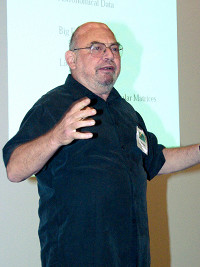
\includegraphics[width=4.5cm]{../pic/leo_breiman.png}
	Изобретатели Случайного Леса (Random Forest):
	\begin{itemize}
		\item Павлов Юрий Леонидович (р.1949)
		\item Лео Брейнман (Leo Breiman) (1928 — 2005)
	\end{itemize}
\end{frame}
  
\section{Список материалов}
  
  \begin{frame}{Случайные леса}
  Сергей Павлович Чистяков \textbf{<<Случайные леса: обзор>>}\footnote{\tiny
\url{http://resources.krc.karelia.ru/transactions/doc/trudy2013/trudy_2013_1_117-136.pdf}
}

	\textbf{sklearn}:
	\begin{itemize}
		\item sklearn.ensemble.RandomForestClassifier\footnote{
			\tiny \url{https://scikit-learn.org/stable/modules/generated/sklearn.ensemble.RandomForestClassifier.html}
		}
		\item sklearn.ensemble.RandomForestRegressor\footnote{
			\tiny
			\url{https://scikit-learn.org/stable/modules/generated/sklearn.ensemble.RandomForestRegressor.html}
		}
	    \item sklearn.ensemble.IsolationForest\footnote{
	       \tiny
	       \url{https://scikit-learn.org/stable/modules/generated/sklearn.ensemble.IsolationForest.html}
    	}
	\end{itemize}
  \end{frame}
  
  \section{Вопросы к лекции}
  
  \begin{frame}
  В банковской системе <<ВашБанк Онлайн>> введена система фрод-мониторинга. 
  Она представляет собой лес решений из 700 деревьев решений. Функция принятия решений -- среднее арифметическое. На определённой транзакции 573 деревьев определило транзакцию как мошенническую, 57 как легитимную, остальные -- отказ от классификации.
  \begin{enumerate}
     \item каков отклик системы ФМ?
     \item каков отклик системы ФМ, если отказ от классификации считать легитимными операциями?
     \item каков отклик системы ФМ, если отказ от классификации считать подозрением на мошенничество?
     \item каков отклик системы ФМ, если отказ от классификации считать подозрением на мошенничество, однако вклад брать не как 1, а как 0.7 ?
  \end{enumerate}
  
  \end{frame}


\begin{frame}{Индекс Джини и бины}
	\begin{enumerate}
		\item Почему на практике используют индекс Джини, а не энтропию по Шеннону? 
		Можете придумать ещё более простую меру загрязнённости, чем индекс Джини?
		\item При каких условиях индекс Джини равен нулю? При каких 1/2 ? 
		При каких равен 1? При каких условиях не определён?
		\item Докажите что для любого количества классов $n$, индекс Джини лежит в границах: $\delta \in [0, \frac{1}{2}]$.
		\item Почему бины обязательно квадратные, а не круглые или треугольные? Какая разница
		в каком подпространстве признаков рассчитывать индекс Джини? 	
	\end{enumerate}
\end{frame}



\begin{frame}{Случайное дерево. Случайный лес.}
	\begin{enumerate}
	\item С помощью кванторов и слов 
	напишите строгий академический алгоритм,
	описывающий построение случайного дерева 
	над пространством признаков $R^n$.
	\item Аналогично п.1, напишите 
	строгий академический алгоритм,
	описывающий построение случайного леса
	\end{enumerate} 
\end{frame} 
  

\end{document}